% =============================================================================
% TEMPLATE DE ARTIGO - PROJETO DE PESQUISA EM COMPUTAÇÃO GRÁFICA
% Bacharelado em Ciência da Computação - IFNMG - Campus Montes Claros
% Disciplina: Computação Gráfica - 2026/2
% Professor: Wagner Ferreira de Barros
%
% Formato didático inspirado em características recorrentes de conferências de
% Computação Gráfica (p.ex., ACM SIGGRAPH/SIGGRAPH Asia e Eurographics):
% texto compacto, duas colunas, corpo em 9 pt, pequeno espaçamento vertical e
% figuras/tabelas integradas ao fluxo.
%
% IMPORTANTE: este é o modelo oficial DA DISCIPLINA, não o template oficial de
% um evento específico. Para futura submissão, migre o conteúdo para o template
% oficial do evento escolhido e siga integralmente as regras daquela chamada.
%
% Extensão exigida na disciplina: 8 a 12 páginas, incluindo referências.
% =============================================================================

\documentclass[9pt,a4paper,twocolumn]{extarticle}

% -----------------------------------------------------------------------------
% Codificação, idioma e tipografia
% -----------------------------------------------------------------------------
\usepackage[T1]{fontenc}
\usepackage[utf8]{inputenc}
\usepackage[brazil]{babel}
\usepackage{newtxtext,newtxmath}
\usepackage{microtype}

% -----------------------------------------------------------------------------
% Página e colunas
% Área útil próxima aos padrões compactos usados em publicações de CG.
% -----------------------------------------------------------------------------
\usepackage[a4paper,textwidth=177mm,textheight=245mm,centering]{geometry}
\setlength{\columnsep}{8mm}
\setlength{\columnseprule}{0pt}
\setlength{\parindent}{1em}
\setlength{\parskip}{0pt}
\linespread{0.97}
\pagestyle{empty}

% -----------------------------------------------------------------------------
% Seções compactas
% -----------------------------------------------------------------------------
\usepackage{titlesec}
\titleformat{\section}
  {\normalfont\bfseries\fontsize{10.5}{11.5}\selectfont}
  {\thesection}{0.5em}{}
\titleformat{\subsection}
  {\normalfont\bfseries\fontsize{9.5}{10.5}\selectfont}
  {\thesubsection}{0.45em}{}
\titlespacing*{\section}{0pt}{7pt plus 2pt minus 1pt}{3pt}
\titlespacing*{\subsection}{0pt}{5pt plus 1pt minus 1pt}{2pt}

% -----------------------------------------------------------------------------
% Figuras, tabelas, matemática e listas
% -----------------------------------------------------------------------------
\usepackage{graphicx}
\usepackage{booktabs}
\usepackage{tabularx}
\usepackage{array}
\usepackage{amsmath}
\usepackage{siunitx}
\usepackage{subcaption}
\usepackage{balance}
\usepackage{enumitem}
\setlist[itemize]{leftmargin=1.25em,itemsep=0pt,topsep=2pt,parsep=0pt}
\setlist[enumerate]{leftmargin=1.5em,itemsep=0pt,topsep=2pt,parsep=0pt}

% -----------------------------------------------------------------------------
% Legendas compactas
% -----------------------------------------------------------------------------
\usepackage[font=small,labelfont=bf]{caption}
\captionsetup{skip=3pt}
\setlength{\textfloatsep}{7pt plus 2pt minus 2pt}
\setlength{\floatsep}{6pt plus 2pt minus 2pt}
\setlength{\intextsep}{6pt plus 2pt minus 2pt}

% -----------------------------------------------------------------------------
% Referências e links
% -----------------------------------------------------------------------------
\usepackage[backend=biber,style=authoryear,maxcitenames=2,maxbibnames=20]{biblatex}
\addbibresource{referencias.bib}
\usepackage[hidelinks]{hyperref}
\usepackage{url}

% -----------------------------------------------------------------------------
% Código-fonte
% -----------------------------------------------------------------------------
\usepackage{xcolor}
\usepackage{listings}
\definecolor{codegray}{gray}{0.45}
\definecolor{codegreen}{rgb}{0.0,0.40,0.0}
\definecolor{codeblue}{rgb}{0.10,0.20,0.65}
\lstset{
  basicstyle=\ttfamily\scriptsize,
  keywordstyle=\color{codeblue}\bfseries,
  commentstyle=\color{codegreen},
  numberstyle=\tiny\color{codegray},
  numbers=left,
  numbersep=4pt,
  frame=single,
  aboveskip=4pt,
  belowskip=4pt,
  breaklines=true,
  showstringspaces=false,
  columns=fullflexible
}

% -----------------------------------------------------------------------------
% Orientações didáticas
% Troque para \mostrarorientacoesfalse antes da entrega final.
% -----------------------------------------------------------------------------
\newif\ifmostrarorientacoes
\mostrarorientacoestrue

\newcommand{\orientacao}[1]{%
  \ifmostrarorientacoes
    \par\smallskip
    \noindent\fcolorbox{black!35}{black!4}{%
      \parbox{0.94\columnwidth}{\fontsize{7.4}{8.2}\selectfont\textbf{Orientação aos autores:} #1}%
    }%
    \par\smallskip
  \fi
}


% -----------------------------------------------------------------------------
% Acréscimos da equipe ao preâmbulo
% -----------------------------------------------------------------------------
\usepackage{pgfplots}
\pgfplotsset{compat=1.17}

% Marca trechos ainda não redigidos. Remover todas as ocorrências antes da entrega.
\newcommand{\pendente}[1]{{\color{red!70!black}\textbf{[PENDENTE:} #1\textbf{]}}}

% =============================================================================
% DOCUMENTO
% =============================================================================
\begin{document}

\twocolumn[
\begin{center}
  {\sffamily\bfseries\fontsize{14}{16}\selectfont
   Otimização do Consumo de Memória no Cálculo da Distância de
   Pompeiu-Hausdorff com Busca de Aprofundamento Iterativo (IDA*)\par}
  \vspace{5pt}
  {\fontsize{9.5}{11}\selectfont
   Stefano Lopes Delgado \quad Pedro Bazzarella Pereira \quad Matheus Antunes Freire
   \par}
  \vspace{2pt}
  {\fontsize{8.5}{10}\selectfont
   Instituto Federal do Norte de Minas Gerais -- IFNMG, Campus Montes Claros\par
   \texttt{sld2@aluno.ifnmg.edu.br pbp1@aluno.ifnmg.edu.br maf6@aluno.ifnmg.edu.br}\par}
\end{center}
\vspace{3pt}

\begin{minipage}{0.94\textwidth}
\fontsize{8.5}{9.5}\selectfont
\noindent\textbf{Resumo.}
O método de Sacht e Jacobson aproxima a distância de Pompeiu-Hausdorff entre
sopas de triângulos com tolerância garantida usando branch and bound com uma
cascata de quatro cotas superiores e uma busca best-first apoiada em uma fila de
prioridade global. Investigamos a substituição dessa busca por uma busca de
aprofundamento iterativo com ramificação e poda (IDA*), que mantém a mesma
cascata de cotas e o mesmo critério de parada. Em resultados preliminares com
três pares de malhas e duas tolerâncias, o IDA* reduziu o pico de memória
residente em 83\% a 86\% nas malhas pequenas e médias e em cerca de 21\% no
modelo Lucy (28 milhões de faces), ao custo de 1,9 a 21,6 vezes mais tempo nas
malhas pequenas e médias, devido à reexpansão de triângulos.
\pendente{atualizar com os resultados finais}

\vspace{3pt}
\noindent\textbf{Palavras-chave:} distância de Pompeiu-Hausdorff; malhas triangulares;
branch and bound; aprofundamento iterativo; consumo de memória.

\vspace{5pt}
\noindent\textbf{Abstract.}
Sacht and Jacobson approximate the Pompeiu-Hausdorff distance between triangle
soups up to a guaranteed tolerance using branch and bound with four cascading
upper bounds and a best-first search driven by a global priority queue. We
replace this search with an iterative-deepening branch and bound (IDA*) that
keeps the same cascade of bounds and stopping criterion, and we measure the
resulting trade-off between peak memory and running time.
\pendente{complete with final results}

\vspace{3pt}
\noindent\textbf{Keywords:} Pompeiu-Hausdorff distance; triangle meshes;
branch and bound; iterative deepening; memory footprint.
\end{minipage}
\vspace{8pt}
]

% =============================================================================
\section{Introdução}
% =============================================================================
\orientacao{Contextualize o problema de Computação Gráfica, explique sua relevância,
apresente o trabalho de referência e conduza o leitor até a questão específica investigada.
A introdução deve terminar com a questão/hipótese e as contribuições do artigo.}

A distância de Pompeiu-Hausdorff unilateral entre duas superfícies $A$ e $B$,
\begin{equation}
  h(A,B) = \max_{p \in A} d(p, B), \qquad d(p,B) = \min_{q \in B} \lVert p - q \rVert,
  \label{eq:hausdorff}
\end{equation}
é a maior distância de um ponto de $A$ até $B$. Em Computação Gráfica, ela é usada
para formular e validar métodos de simplificação, remalhamento e geração de malhas,
em geral quando $A$ e $B$ representam o mesmo objeto e se deseja certificar que a
diferença entre elas é pequena~\parencite{sacht2024cascading}. Calcular $h(A,B)$
com precisão garantida é difícil porque o maximizador pode estar no interior de
qualquer triângulo de $A$.

Sacht e Jacobson~\parencite{sacht2024cascading} aproximam $h(A,B)$ até uma tolerância
$\varepsilon$ com branch and bound e uma cascata de quatro cotas superiores, obtendo
o método preciso mais rápido da literatura. A busca é best-first: todos os triângulos
ativos ficam em uma fila de prioridade ordenada pela cota superior, e um parâmetro
$m$ limita o número de triângulos processados para controlar a memória.

\textbf{Questão investigada.} Substituir a busca best-first por uma busca de
aprofundamento iterativo com ramificação e poda (IDA*)~\parencite{korf1985depth}
reduz o pico de memória do método, preservando a garantia de tolerância? Qual é o
custo em tempo de execução?

\textbf{Contribuições.} \pendente{revisar ao final}
\begin{itemize}
  \item reprodução da baseline a partir do código público dos autores e
        modularização da rotina de busca em motores intercambiáveis;
  \item implementação de um motor IDA* que reutiliza a cascata de cotas original;
  \item avaliação experimental do compromisso entre memória e tempo em malhas de
        tamanhos diferentes.
\end{itemize}

% =============================================================================
\section{Trabalho de Referência e Trabalhos Relacionados}
% =============================================================================
\orientacao{Apresente o artigo-base com precisão suficiente para que o leitor entenda
a técnica que será modificada. Discuta apenas a literatura necessária para posicionar
a proposta. Verifique trabalhos posteriores antes de afirmar novidade.}

\subsection{Branch and bound para a distância de Pompeiu-Hausdorff}
Métodos precisos~\parencite{tang2009interactive,kang2018fast,zheng2022economic}
mantêm uma cota inferior global $l$, dada pela maior distância de um vértice de $A$
até $B$, e uma cota superior $u_t$ para cada triângulo $t$ de $A$. Triângulos com
$u_t < l$ não contêm o maximizador e são descartados; os demais são subdivididos em
quatro pelos pontos médios das arestas, o que gera novos vértices que podem aumentar
$l$. O processo termina quando $\max_t u_t - l \le \varepsilon$.
\pendente{detalhar diferenças entre TLK09, KKYK18 e ZSL22}

\subsection{Cotas superiores em cascata}
Sacht e Jacobson~\parencite{sacht2024cascading} avaliam quatro cotas superiores em
ordem crescente de custo e precisão: \pendente{descrever $u_1$ a $u_4$ em uma frase
cada}. Um triângulo é descartado assim que alguma cota fica abaixo de $l$, de modo
que a maioria dos triângulos é eliminada pelas cotas mais baratas. No conjunto de
testes completo, o método foi 16 vezes mais rápido que o de Zheng et
al.~\parencite{zheng2022economic}.

\subsection{Busca de aprofundamento iterativo}
O IDA*~\parencite{korf1985depth} combina busca em profundidade com limiares sucessivos
sobre a função de avaliação: cada iteração explora apenas os nós acima do limiar
corrente, e o limiar da iteração seguinte é o melhor valor deixado de fora. A memória
é proporcional à profundidade da busca, ao custo de reexpandir nós a cada iteração.
\pendente{verificar trabalhos que usam IDA* ou DFBnB em consultas geométricas}

% Figura de largura total declarada antes do ponto em que é citada: o LaTeX a
% posiciona no topo da página seguinte. Declarada perto do fim, ela é descartada
% pelo \balance junto com os floats de uma coluna.
\begin{figure*}[t]
\centering
\begin{subfigure}[b]{0.22\textwidth}
  \centering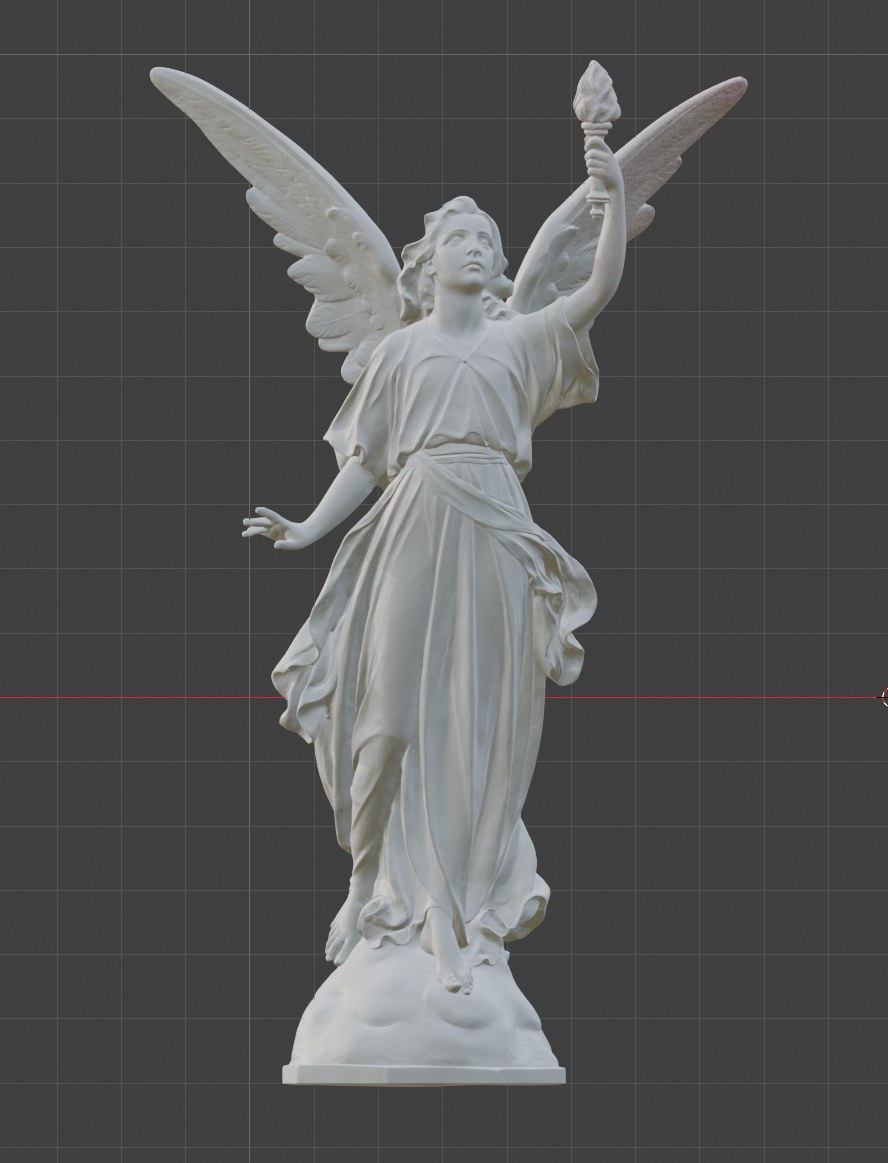
\includegraphics[height=4.2cm]{figuras/lucy_original.jpg}
  \caption{Lucy original.}
\end{subfigure}\hfill
\begin{subfigure}[b]{0.37\textwidth}
  \centering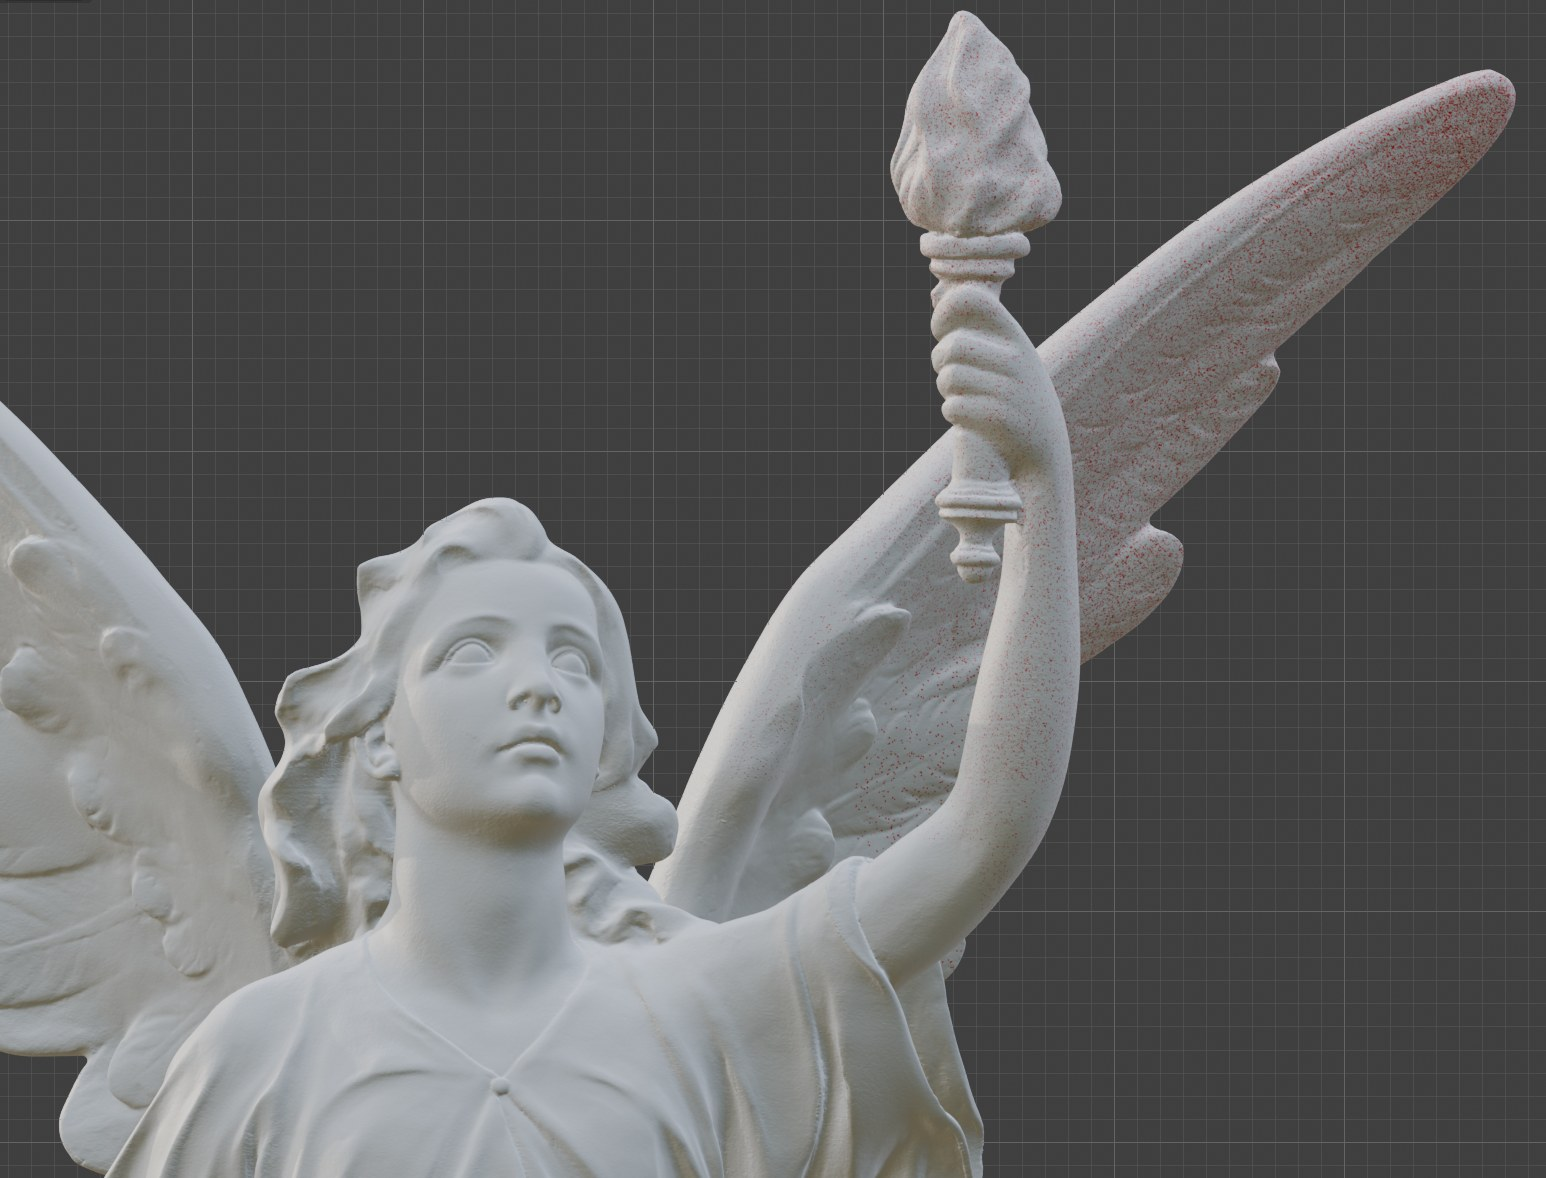
\includegraphics[height=4.2cm]{figuras/lucy_sobreposta.jpg}
  \caption{Original sobreposta à decimada.}
\end{subfigure}\hfill
\begin{subfigure}[b]{0.37\textwidth}
  \centering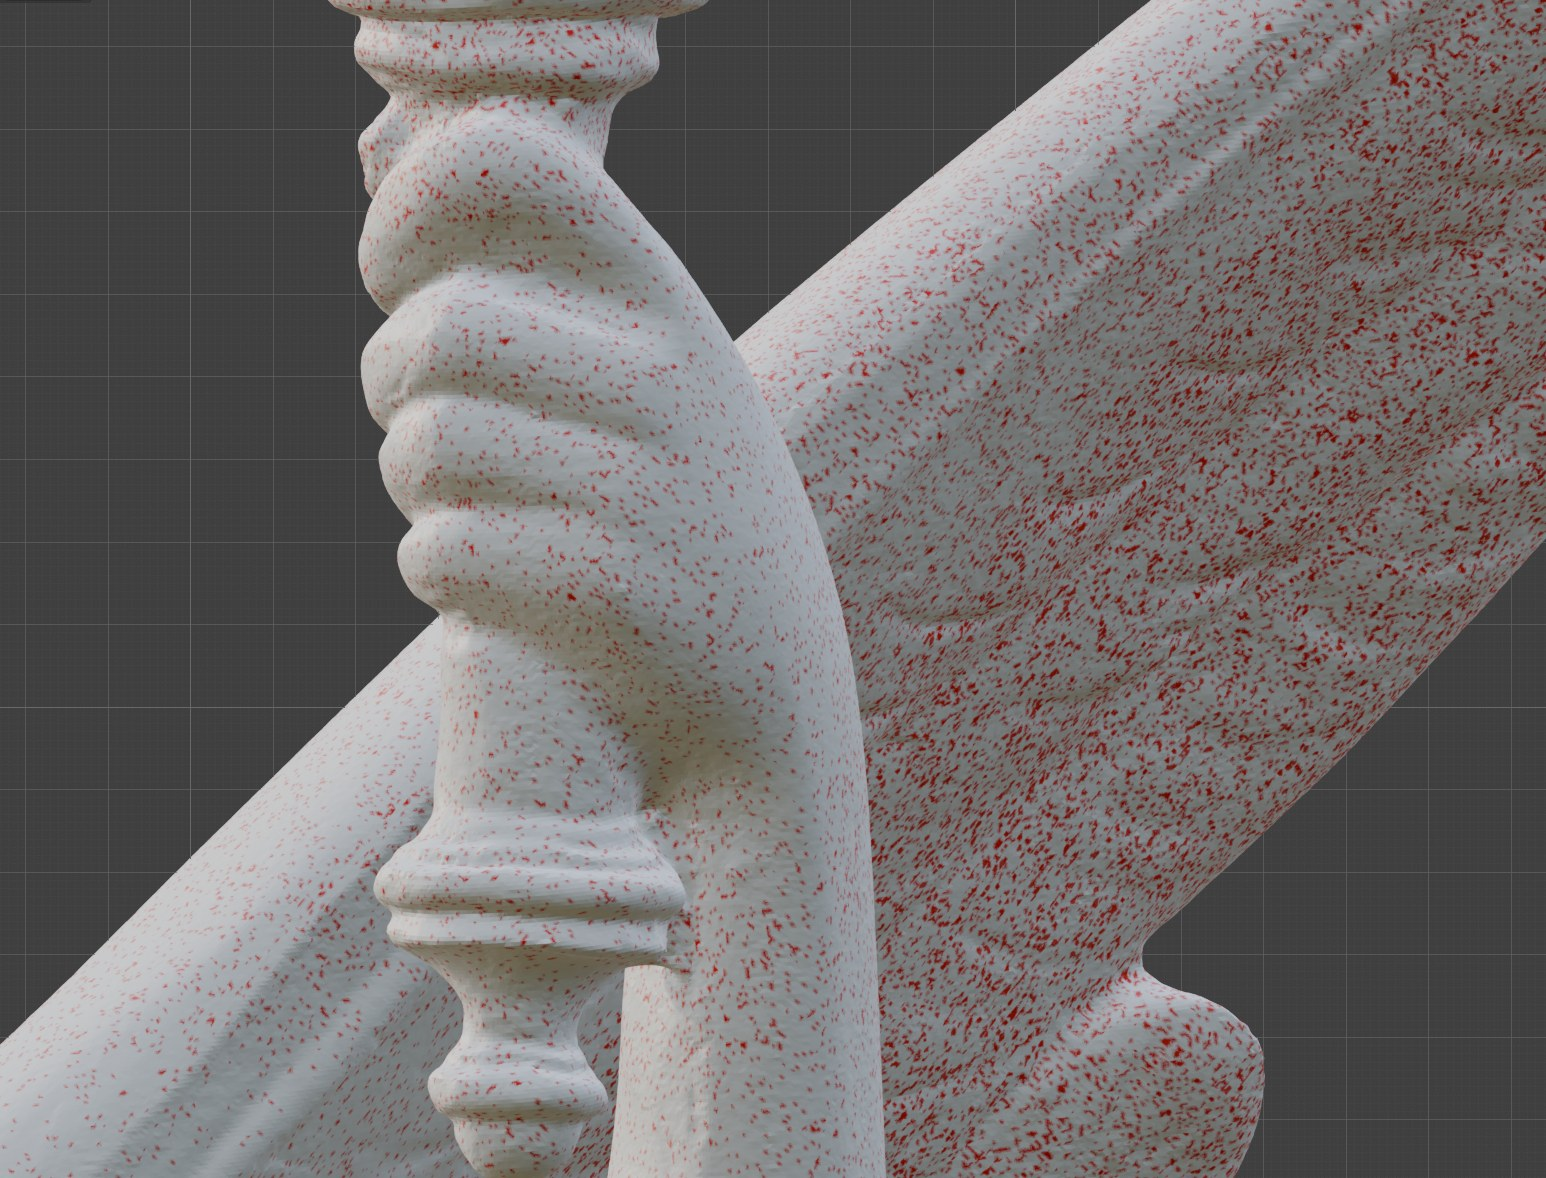
\includegraphics[height=4.2cm]{figuras/lucy_sobreposta_zoom.jpg}
  \caption{Detalhe da sobreposição.}
\end{subfigure}
\caption{Par de malhas Lucy usado nos testes, visualizado no Blender. Nas imagens (b)
e (c), a malha original aparece em vermelho e a decimada em branco; como estão muito
próximas, elas se alternam ao longo de toda a superfície, o que torna difícil
localizar o maximizador de $h(A,B)$.}
\label{fig:lucy}
\end{figure*}

% =============================================================================
\section{Proposta}
% =============================================================================
\orientacao{Descreva exatamente o que foi alterado, acrescentado ou investigado.
Diferencie o método original da contribuição da equipe. Use diagramas, pseudocódigo
ou equações quando melhorarem a reprodutibilidade.}

Mantemos inalterados a estrutura AABB sobre $B$, a cascata de cotas, a subdivisão
1-para-4 e o critério de parada. Alteramos apenas a ordem de exploração e o
armazenamento dos triângulos ativos.

\textbf{Baseline (best-first).} A cada passo, retira-se da fila o triângulo de maior
cota superior, que é subdividido; os filhos com $u \ge l$ são inseridos na fila. A
memória cresce com o número de triângulos ativos e, na implementação original,
também com todos os vértices e faces gerados, que são mantidos em vetores
aumentados.

\textbf{Proposta (IDA*).} Seja $U$ a maior cota superior ainda não refinada. Cada
iteração define um limiar
\begin{equation}
  \theta = U - \max\!\left(\varepsilon,\ \tfrac{1}{4}(U - l)\right)
  \label{eq:limiar}
\end{equation}
e percorre, em profundidade, cada triângulo original com $u > \theta$. Durante o
percurso, um nó é (i) descartado se $u < l$; (ii) adiado se $u \le \theta$, e seu
valor candidata-se ao próximo limiar; (iii) aceito se $u - l \le \varepsilon$; ou
(iv) subdividido, com os filhos visitados em ordem decrescente de cota. Ao fim da
iteração, $U$ recebe o maior valor adiado ou aceito, e a busca termina quando
$U - l \le \varepsilon$. Como nenhum nó é armazenado fora da pilha de recursão, a
memória da busca é $O(d)$, em que $d$ é a profundidade máxima de subdivisão, contra
$O(w)$ da fila best-first, em que $w$ é a largura da fronteira.
\pendente{provar/argumentar que a cota inferior e a cota superior final continuam válidas}

% =============================================================================
\section{Implementação}
% =============================================================================
\orientacao{Informe apenas os detalhes necessários para compreender e reproduzir o
trabalho: linguagem, bibliotecas, versão da baseline, alterações relevantes, hardware
e parâmetros. O manual completo de instalação deve ficar no README do GitHub.}

Partimos do código público dos autores (C++, Eigen, libigl~\parencite{libigl} e CGAL,
licença MPL~2.0). A rotina de busca foi isolada em uma interface
\texttt{DistanceSearchEngine} com duas implementações: \texttt{BestFirstEngine}, que
reproduz o algoritmo original, e \texttt{IDAStarEngine}, a proposta. O motor é
escolhido por argumento de linha de comando. Contadores de triângulos subdivididos e
de chamadas a cada cota foram acrescentados aos dois motores.
\pendente{commit/tag da baseline; versões de compilador e bibliotecas}

\begin{lstlisting}[language=C++,caption={Núcleo recursivo do motor IDA* (simplificado).},label={lst:dfs}]
void dfs(Node n, double theta, double& next) {
  if (n.u < lower) return;                  // poda definitiva
  if (n.u <= theta) { next = max(next, n.u); return; } // adiado
  if (n.u - lower <= tol) { next = max(next, n.u); return; }
  auto kids = subdivide_1_to_4(n);           // atualiza lower
  cascading_bounds(kids, lower);             // u1..u4
  sort_desc_by_upper(kids);
  for (auto& k : kids) if (k.u >= lower) dfs(k, theta, next);
}
\end{lstlisting}

% =============================================================================
\section{Metodologia Experimental}
% =============================================================================
\orientacao{Explique como a hipótese será testada. Identifique baseline, dados/cenas,
parâmetros, métricas, quantidade de execuções, sementes e regras de comparação. Baseline
e proposta devem ser avaliadas sob condições equivalentes.}

\subsection{Questão experimental}
Verificar se o IDA* obtém as mesmas cotas que a baseline, dentro de $\varepsilon$,
com pico de memória menor, e quantificar o custo em tempo.

\subsection{Baseline e variantes}
Baseline: \texttt{BestFirstEngine}, idêntico ao algoritmo original. Proposta:
\texttt{IDAStarEngine}. Os dois motores usam o mesmo binário, as mesmas entradas e os
mesmos parâmetros ($m = 10^6$, tolerância normalizada pela diagonal da caixa
envolvente de $A$).
\pendente{avaliar uma variante best-first que armazene só a fronteira, para separar o
efeito da estratégia de busca do efeito da pré-alocação}

\subsection{Dados, modelos ou cenas}
\begin{itemize}
  \item \textbf{107100}: modelo do Thingi10K~\parencite{zhou2016thingi10k}
        (4\,560 faces) e sua versão remalhada pelo TetWild~\parencite{hu2018tetwild}
        (28\,196 faces), exemplo fornecido pelos autores;
  \item \textbf{848343} (caso médio): modelo do Thingi10K e versão decimada
        \pendente{número de faces e procedimento de decimação};
  \item \textbf{Lucy}~\parencite{stanford3dscan}: 28\,055\,728 faces, e versão
        decimada com 14\,027\,864 faces (Figura~\ref{fig:lucy})
        \pendente{procedimento de decimação}.
\end{itemize}
\pendente{ampliar para 10 a 15 pares de malhas}


\subsection{Métricas e protocolo}
Pico de memória residente (VmHWM em \texttt{/proc} e \texttt{getrusage}), tempo de
parede e de CPU, número de triângulos subdivididos, chamadas a cada cota e cotas
inferior e superior finais. Tolerâncias $\varepsilon \in \{10^{-4}, 10^{-8}\}$.
Os resultados dos dois motores são considerados equivalentes quando ambos os
intervalos satisfazem $u - l \le \varepsilon\, d_A$, em que $d_A$ é a diagonal da
caixa envolvente de $A$, e se sobrepõem.
Cada execução roda em um processo isolado, coordenado pelo script
\texttt{benchmarks/compare\_engines.py}.
\pendente{hardware e SO; repetições (mín.\ 3) com média e desvio padrão;
acrescentar $\varepsilon = 10^{-2}$ e $10^{-3}$}

% =============================================================================
\section{Resultados}
% =============================================================================
\orientacao{Apresente resultados quantitativos e visuais. Toda tabela e figura deve ser
citada no texto e responder a uma questão experimental. Evite imagens meramente decorativas.}

A Tabela~\ref{tab:preliminar} resume os resultados preliminares (uma execução por
configuração). Em cinco das seis configurações, os dois motores obtiveram cotas
idênticas. No par 848343 com $\varepsilon = 10^{-8}$, a cota inferior coincidiu e a
superior diferiu, mas os dois intervalos satisfazem a tolerância
($\varepsilon\, d_A = 1{,}90\times10^{-6}$): $1{,}80\times10^{-6}$ no IDA* e
$2{,}2\times10^{-7}$ na baseline. O IDA* para assim que atinge a tolerância, enquanto
o último passo da baseline termina com folga.

\begin{table}[t]
\caption{Resultados preliminares: pico de memória residente (MB), tempo de parede (s)
e triângulos subdivididos (milhares). BF: best-first (baseline). Uma execução por
configuração.}
\label{tab:preliminar}
\centering
\scriptsize
\setlength{\tabcolsep}{3pt}
\begin{tabular}{llrrrrrr}
\toprule
 & & \multicolumn{2}{c}{Memória (MB)} & \multicolumn{2}{c}{Tempo (s)} & \multicolumn{2}{c}{Subdiv. (mil)} \\
\cmidrule(lr){3-4}\cmidrule(lr){5-6}\cmidrule(lr){7-8}
Par & $\varepsilon$ & BF & IDA* & BF & IDA* & BF & IDA* \\
\midrule
107100 & $10^{-4}$ & 132,5  & 20,0   & 3,2   & 14,1  & 400 & 2\,779 \\
107100 & $10^{-8}$ & 142,5  & 20,0   & 3,3   & 71,5  & 451 & 16\,480 \\
848343 & $10^{-4}$ & 360,1  & 60,4   & 12,0  & 22,7  & 916 & 3\,720 \\
848343 & $10^{-8}$ & 441,1  & 60,7   & 15,6  & 75,7  & 1\,374 & 14\,280 \\
Lucy   & $10^{-4}$ & 5\,993 & 4\,731 & 214,3 & 211,4 & 33  & 130 \\
Lucy   & $10^{-8}$ & 6\,009 & 4\,715 & 203,2 & 258,3 & 66  & 1\,929 \\
\bottomrule
\end{tabular}
\end{table}

A Figura~\ref{fig:razoes} mostra a variação relativa de memória e de tempo do IDA* em
relação à baseline. Nas malhas pequenas e médias, a memória caiu de 83\% a 86\% e o
pico do IDA* ficou praticamente constante entre as tolerâncias (20,0~MB no par
107100), enquanto o da baseline cresceu. O tempo, por outro lado, aumentou de 1,9 a
21,6 vezes, acompanhando o número de triângulos subdivididos (4 a 37 vezes mais, por
causa da reexpansão). Na Lucy, a redução foi de cerca de 21\% (1,26 a 1,29~GB) e o
tempo variou de $-1\%$ a $+27\%$.

\begin{figure}[t]
\centering
\begin{tikzpicture}
\begin{axis}[
  ybar, width=\columnwidth, height=4.2cm,
  bar width=5pt,
  ylabel={IDA* / BF},
  ymode=log, log origin=infty,
  ymin=0.1, ymax=30,
  ytick={0.1,1,10}, yticklabels={{0{,}1},1,10},
  symbolic x coords={107100-4,107100-8,848343-4,848343-8,Lucy-4,Lucy-8},
  xticklabels={{107100\\$10^{-4}$},{107100\\$10^{-8}$},{848343\\$10^{-4}$},{848343\\$10^{-8}$},{Lucy\\$10^{-4}$},{Lucy\\$10^{-8}$}},
  xtick=data, xticklabel style={font=\tiny, align=center},
  yticklabel style={font=\tiny}, ylabel style={font=\scriptsize},
  legend style={font=\tiny, at={(0.5,1.03)}, anchor=south, legend columns=2, draw=none},
  extra y ticks={1}, extra y tick labels={}, extra y tick style={grid=major, grid style={dashed,gray}},
]
\addplot coordinates {(107100-4,0.151) (107100-8,0.140) (848343-4,0.168) (848343-8,0.138) (Lucy-4,0.789) (Lucy-8,0.785)};
\addplot coordinates {(107100-4,4.40) (107100-8,21.59) (848343-4,1.89) (848343-8,4.85) (Lucy-4,0.99) (Lucy-8,1.27)};
\legend{Memória, Tempo}
\end{axis}
\end{tikzpicture}
\caption{Razão IDA*/best-first do pico de memória e do tempo de parede (escala
logarítmica; abaixo de 1, o IDA* é melhor).}
\label{fig:razoes}
\end{figure}

\pendente{figura com a malha $A$, o par maximizador e o mapa de profundidade de subdivisão}

% =============================================================================
\section{Discussão}
% =============================================================================

% =============================================================================
\section{Conclusão}
% =============================================================================

% =============================================================================
% REFERÊNCIAS
% =============================================================================
\balance
\printbibliography[title={Referências}]

\end{document}
